\documentclass[a4paper,12pt]{article}
\usepackage{amsmath}
\usepackage{graphicx}
\usepackage{hyperref}
\usepackage{biblatex}
\usepackage{minted}

\addbibresource{M3-Eduardo-Bayot.bib} % Archivo .bib para las referencias


\begin{document}

% Carátula
\begin{titlepage}
    \begin{center}
        
\includegraphics[width=0.3\textwidth]{logo.png}\\[1cm] % Inserta el logo aquí, ajusta la ruta si es necesario
        \textsc{\LARGE Universidad Siglo 21}\\[1.5cm]
        \textsc{\Large Trabajo Práctico Nro 3}\\[0.5cm]
        \textsc{\large Estadística y Probabilidad}\\[2cm]

        \rule{\linewidth}{0.5mm} \\[0.4cm]
        {\huge \bfseries Validación de Hipótesis Estadísticas}\\[0.4cm]
        \rule{\linewidth}{0.5mm} \\[1.5cm]

        \begin{tabular}{rl}
            \small Profesor Titular Experto: & \small Yanina Nancy Morales \\
            \small Profesor Titular Disciplinar: & \small Horacio José Caballero \\
        \end{tabular}
        \\[1.5cm]

        \textbf{\small Estudiante: Eduardo Bayot}\\
        \textbf{\small Cátedra: D}\\
        \textbf{\small Grupo: 1}
    \end{center}
\end{titlepage}

% Reiniciar numeración después de la carátula
\pagenumbering{arabic}


% Configuración de la página
\date{}
\author{}

\tableofcontents




\tableofcontents

\section{Introducción}

En este trabajo práctico se analiza una situación estadística relacionada con la validación de afirmaciones realizadas por un fabricante sobre la temperatura de activación de un sistema de rociadores contra incendios. Según el fabricante, la temperatura promedio de activación es de 130°F. Este análisis tiene como objetivo verificar dicha afirmación mediante una prueba de hipótesis estadística.

Se utiliza la metodología planteada en el módulo de Probabilidad y Estadística, empleando simulaciones generadas en el software R para replicar una muestra de datos basada en una distribución normal con parámetros específicos. La validación se realizará evaluando si los datos obtenidos contradicen la hipótesis nula planteada a un nivel de significancia del 1\%.

La introducción al análisis se fundamenta en los conceptos de pruebas de hipótesis, regiones de rechazo y estadísticos de prueba. Este trabajo busca responder a la pregunta de si los datos muestrales proporcionan evidencia suficiente para rechazar la afirmación del fabricante o si no existen razones suficientes para contradecirla. Finalmente, los resultados serán interpretados para concluir si la hipótesis del fabricante es consistente con los datos simulados.


\section{Metodología}

El desarrollo de este trabajo se estructura en tres etapas principales: planteo del problema, simulación de datos y aplicación de una prueba de hipótesis para evaluar la validez de la afirmación del fabricante. A continuación, se describe cada una de estas etapas.

\subsection{Planteo del Problema}
El problema planteado consiste en validar la afirmación del fabricante de que la temperatura promedio de activación de los sistemas de rociadores es de 130°F. Para ello, se define la hipótesis nula (\(H_0\)) y la hipótesis alternativa (\(H_a\)):

\begin{itemize}
    \item \(H_0: \mu = 130\), donde \(\mu\) es la temperatura promedio de activación.
    \item \(H_a: \mu \neq 130\), lo que indica que la temperatura promedio de activación difiere de 130°F.
\end{itemize}

Esta prueba se llevará a cabo con un nivel de significancia de \( \alpha = 0.01 \), utilizando un enfoque bilateral dado que la hipótesis alternativa no especifica una dirección particular en el cambio.

\subsection{Simulación de Datos en R}
Los datos muestrales serán generados utilizando el software R. Según lo especificado en la consigna, la muestra se obtiene utilizando la función \texttt{rnorm}, que genera valores aleatorios de una distribución normal con media \(\mu = 130\) y desviación estándar \(\sigma = c\), donde \(c\) es el tercer dígito no nulo del DNI. El tamaño de la muestra (\(n\)) es determinado por la suma de los dos primeros dígitos no nulos del DNI.

La generación de datos mediante simulaciones permite replicar el comportamiento de un experimento real de forma controlada. Según Quevedo et al. (2009), las simulaciones son una herramienta poderosa para comprender la variabilidad inherente a los datos y evaluar hipótesis estadísticas bajo diferentes supuestos \cite{quevedo2009}.

\subsection{Prueba de Hipótesis}
Para evaluar la afirmación del fabricante, se utiliza una prueba de hipótesis para la media de una población con desviación estándar conocida, basada en el estadístico \(Z\):

\[
Z = \frac{\overline{X} - \mu_0}{\sigma / \sqrt{n}}
\]

Donde:
\begin{itemize}
    \item \(\overline{X}\) es el promedio muestral.
    \item \(\mu_0\) es el valor bajo la hipótesis nula (130°F).
    \item \(\sigma\) es la desviación estándar de la población (valor \(c\)).
    \item \(n\) es el tamaño de la muestra.
\end{itemize}

La región de rechazo será determinada según los valores críticos de \(Z\) para un nivel de significancia del 1\% en una prueba bilateral. De acuerdo con Quevedo et al. (2009), la correcta definición de estas regiones es crucial para minimizar errores de tipo I y II, asegurando decisiones fundamentadas estadísticamente \cite{quevedo2009}.




\section{Desarrollo}
\subsection{Tabla de Valores Simulados}

En esta subsección se presentan los valores generados a partir de una distribución normal con media \( \mu = 130 \) y desviación estándar \( \sigma = c \), donde los parámetros se calculan a partir del DNI del estudiante. La muestra tiene un tamaño de \( n = 5 \), que corresponde a la suma de los dos primeros dígitos no nulos del DNI (\( a = 3 \) y \( b = 2 \)). Los datos fueron generados en R con el siguiente código:

\begin{minted}{R}
# Configuración del DNI
a <- 3
b <- 2
c <- 4

# Tamaño de la muestra
n <- a + b

# Fijar semilla para reproducibilidad
set.seed(123)

# Generar la muestra
muestra <- rnorm(n, mean = 130, sd = c)

# Mostrar la tabla generada
print(muestra)

# Guardar como data.frame para exportar o analizar
tabla_muestra <- data.frame(Valores = muestra)

# Opcional: exportar a CSV
write.csv(tabla_muestra, "tabla_muestra.csv", row.names = FALSE)
\end{minted}

Los valores obtenidos se presentan en la Tabla \ref{tab:valores_simulados}.

\begin{table}[h!]
\centering
\begin{tabular}{|c|}
\hline
\textbf{Valores Simulados} \\ \hline
127.758 \\ \hline
129.079 \\ \hline
136.235 \\ \hline
130.282 \\ \hline
130.517 \\ \hline
\end{tabular}
\caption{Valores generados a partir de una distribución \(N(130, c)\) con \( n = 5 \) y \( c = 4 \).}
\label{tab:valores_simulados}
\end{table}

\subsection{Planteo de Hipótesis}

El análisis estadístico se centra en evaluar la afirmación del fabricante de que la temperatura promedio de activación de los sistemas de rociadores es de \( \mu = 130 \) grados Fahrenheit. Para ello, se establece un planteo formal de hipótesis, como se describe a continuación:

\begin{itemize}
    \item \textbf{Hipótesis Nula (\( H_0 \))}: \( \mu = 130 \), donde \( \mu \) es la temperatura promedio de activación.
    \item \textbf{Hipótesis Alternativa (\( H_a \))}: \( \mu \neq 130 \), lo que indica que la temperatura promedio de activación es diferente de 130 grados Fahrenheit.
\end{itemize}

La prueba de hipótesis se realiza con un nivel de significancia de \( \alpha = 0.01 \), utilizando un enfoque bilateral. Esto significa que cualquier desviación significativa de la media, ya sea hacia valores mayores o menores, puede llevar al rechazo de la hipótesis nula.

En términos gráficos, la región de rechazo corresponde a los valores del estadístico \( Z \) que caen en las colas de la distribución normal estándar, delimitadas por los valores críticos \( Z_{\alpha/2} \) y \( -Z_{\alpha/2} \). Según Quevedo et al. (2009), la correcta formulación de las hipótesis y la identificación de la región de rechazo son pasos fundamentales para minimizar errores y garantizar resultados confiables \cite{quevedo2009}.

\begin{figure}[h!]
\centering
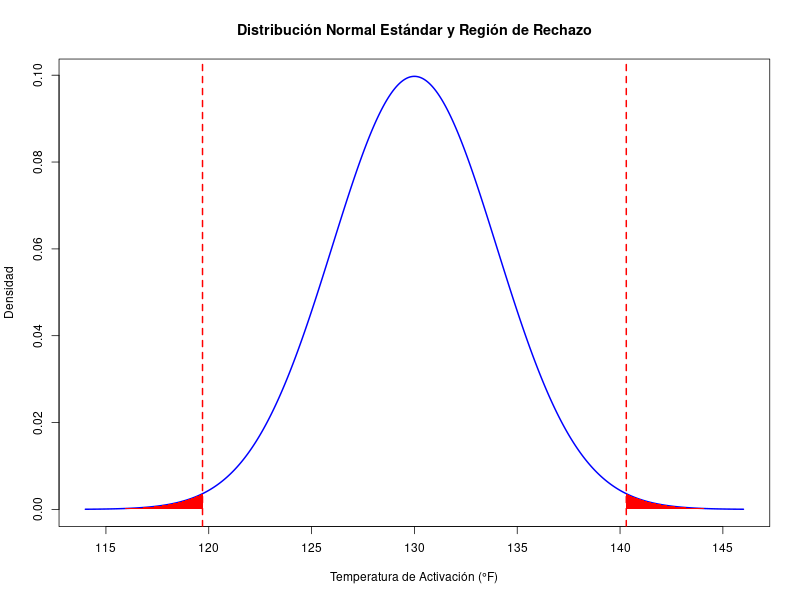
\includegraphics[width=0.8\textwidth]{region_rechazo.png}
\caption{Distribución normal estándar con regiones de rechazo sombreadas. Los valores críticos delimitan las áreas donde se rechaza la hipótesis nula a un nivel de significancia de \( \alpha = 0.01 \).}
\label{fig:region_rechazo}
\end{figure}


\subsection{Cálculo del Estadístico de Prueba}

El estadístico de prueba utilizado para evaluar la hipótesis nula es \( Z \), que mide la distancia entre el promedio muestral (\( \overline{X} \)) y la media poblacional bajo la hipótesis nula (\( \mu_0 \)), en unidades de error estándar. La fórmula utilizada es:

\[
Z = \frac{\overline{X} - \mu_0}{\sigma / \sqrt{n}}
\]

Donde:
\begin{itemize}
    \item \( \overline{X} \): promedio muestral, calculado a partir de los datos simulados.
    \item \( \mu_0 \): media poblacional bajo la hipótesis nula.
    \item \( \sigma \): desviación estándar conocida de la población.
    \item \( n \): tamaño de la muestra.
\end{itemize}

Utilizando los valores obtenidos:
\begin{itemize}
    \item \( \overline{X} = 130.7743 \) (promedio muestral calculado).
    \item \( \mu_0 = 130 \).
    \item \( \sigma = 4 \).
    \item \( n = 5 \).
\end{itemize}

El estadístico \( Z \) se calcula como:

\[
Z = \frac{130.7743 - 130}{4 / \sqrt{5}} = 0.4328
\]

El valor de \( Z = 0.4328 \) indica que la distancia entre el promedio muestral y la media hipotética es de aproximadamente 0.43 desviaciones estándar. Este valor será comparado con los valores críticos de la región de rechazo en la siguiente sección.

\subsection{Determinación de la Región de Rechazo}
Cálculo del valor crítico y comparación con el estadístico.
\subsection{Decisión y Conclusión}
Discusión de los resultados y decisión respecto a \( H_0 \).

\section{Resultados}
Interpretación final de los resultados obtenidos y validación de la afirmación del fabricante.

\section{Referencias}

Las fuentes utilizadas en el presente trabajo son las siguientes:

\begin{itemize}
    \item Quevedo Urias, H., \& Pérez Salvador, B. R. (2009). \textit{Estadística para Ingeniería y Ciencias}. Editorial Patria.
    \item R Core Team. (2023). \textit{The R Project for Statistical Computing}. Recuperado de \url{https://www.r-project.org/}.
\end{itemize}

\printbibliography

\end{document}
